%\renewcommand{\theequation}{\theenumi}
\begin{enumerate}[label=\thesection.\arabic*.,ref=\thesection.\theenumi]
%\numberwithin{equation}{enumi}
\numberwithin{equation}{subsection}
\item We have the values of all three sides of the triangle ABC and PQR so to construct  a triangle we need all three coordinates of A,B and C.After getting the all three coordinates the coordinates of the median from point A to side BC and from point P to line QR, are achieved.


%\renewcommand{\thefigure}{\theenumi.\arabic{figure}}
\begin{figure}[!ht]
\centering
\resizebox{\columnwidth}{!}{\input{./figs/triangle.tex}}
\caption{ Triangles by Latex-Tikz}
\label{fig:con_triangles}	
\end{figure}
%
%
%\renewcommand{\thefigure}{\theenumi}
%


%
\begin{table}[ht!]
\centering
%\begin{tabular}{ |p{3cm}|p{3cm}|  }
%\hline
% \multicolumn{2}{|c|}{Initial Input Values.} \\
%\hline
%a & 4\\
%\hline
%b & 3\\
%\hline
%$\phase{(ACB)$ & $90^{\circ}$ \\
%\hline
%\end{tabular}
\input{./tables/inp.tex}
\caption{To construct $\triangle ACB$ and $\triangle PQR$}
\label{table:table1}	
\end{table}

%\item
%	For simplicity, let the greek letter $\alpha = \phase{ B$.  We have the following definitions.
%\begin{equation}
%\label{eq:tri_trig_defs}
%\begin{matrix}
	%\sin \theta = \frac{b}{c} & 	\cos \theta = \frac{a}{c} \\
	%\tan \theta = \frac{c}{a} & \cot \theta = \frac{1}{\tan \theta} \\
	%\csc \theta = \frac{1}{\sin \theta} & \sec \theta = \frac{1}{\cos \theta}
	%\end{equation}
%
\item Finding out  the coordinates of the various points in Fig. \ref{fig:con_triangles}
\label{const:con_triangles}
\\
% 
%$\triangle ABC$ are 
\begin{align}
\label{eq:constr_a}
x = \frac{\left(a^2 + c^2 - b^2\right)}{2*a}
\\
y = \sqrt{c^2 - x^2}
\\
\vec{A} &= \myvec{x \\ y}
\\
\vec{B} &= \myvec{0 \\ 0}
\\
\label{eq:constr_c}
\vec{C} &= \myvec{a  \\ 0 }
\\
\vec{P} &= \myvec{x+5 \\ y }
\label{eq:constr_b}
\end{align}
Similarly we can get q and r
\\

$\because \vec{M}$ is the midpoint of $BC$ and $\vec{N}$ of $QR$,
\begin{align}
\vec{M} &= \frac{1}{2}\myvec{a\\0}
\\
\vec{N} &= \frac{1}{2}\myvec{a+5\\0}
\end{align}
 
%\item List the  derived values.
%\label{const:table2}
%\\
%\solution See   
\begin{table}[ht!]
\centering
\begin{tabular}{ |p{3cm}|p{3cm}|  }
\hline
 \multicolumn{2}{|c|}{Derived Values.} \\
\hline
$\vec{M}$ & $$\begin{pmatrix}1.5\\0\end{pmatrix}$$\\						
\hline
$\vec{N}$ & $$\begin{pmatrix}6.5\\0\end{pmatrix} $$\\
\hline
\end{tabular}
\caption{To construct madian AM and PN}
\label{table:table2}
\end{table}
%
\item Drawing  Fig. \ref{fig:con_triangles}.	
\\
 The  following Python code generates Fig. \ref{fig:tri_sss_py}
 \\
%
\begin{lstlisting}
./codes/Triangle.py
\end{lstlisting}
\begin{figure}[!ht]
\centering
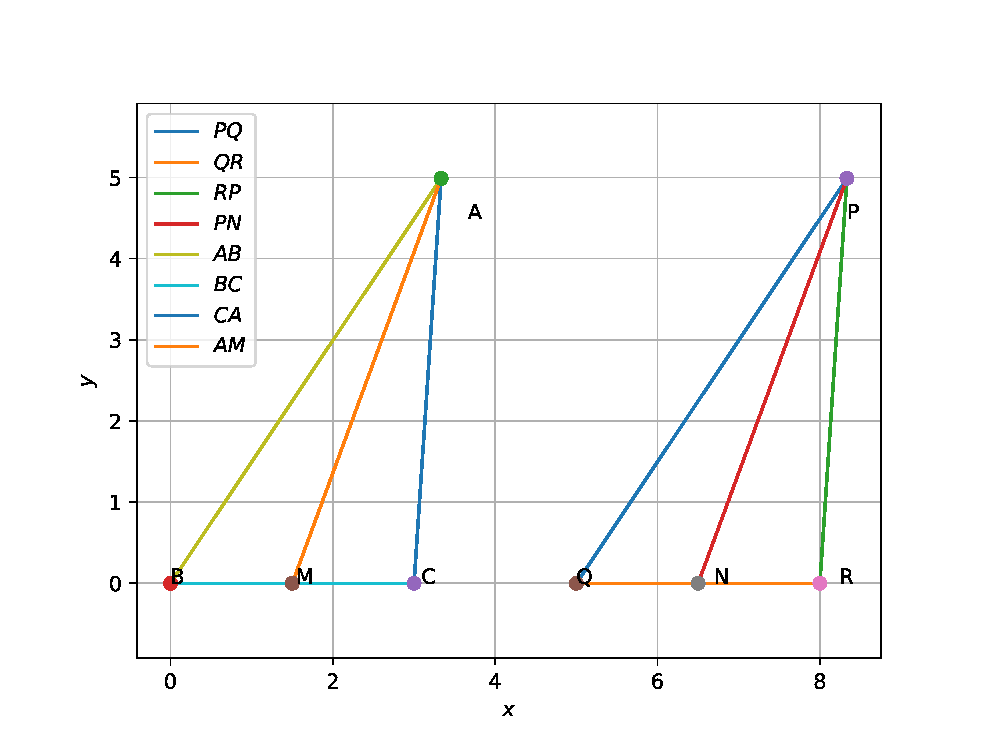
\includegraphics[width=\columnwidth]{./figs/Triangle.eps}
\caption{Triangles generated using python}
\label{fig:tri_sss_py}
\end{figure}

%
and the equivalent latex-tikz code generating Fig.2.1  is 
\begin{lstlisting}
./figs/triangle.tex
\end{lstlisting}
%
The above latex code can be compiled as a standalone document as
\begin{lstlisting}
./figs/triangle_fig.tex
\end{lstlisting}

%

%

%
%

\end{enumerate}

